% Author: Alfredo Sánchez Alberca (asalber@ceu.es)

\chapter{Contraste de Hipótesis}

\section{Fundamentos teóricos}

\subsection{Inferencia Estadística y Contrastes de Hipótesis}

Cualquier afirmación o conjetura que determina, parcial o totalmente, la distribución de una población se realiza
mediante una \emph{Hipótesis Estadística}.

En general, nunca se sabe con absoluta certeza si una hipótesis es cierta o falsa, ya que, para ello tendríamos que
medir a todos los individuos de la población. Las decisiones se toman sobre una base de probabilidad y los
procedimientos que conducen a la aceptación o rechazo de la hipótesis forman la parte de la Inferencia Estadística que
se denomina \emph{Contraste de Hipótesis}.

Una hipótesis se contrasta comparando sus predicciones con la realidad que se obtiene de las muestras: si coinciden,
dentro del margen de error probabilísticamente admisible, mantendremos la hipótesis; en caso contrario, la rechazamos y
buscaremos nuevas hipótesis capaces de explicar los datos observados.

\subsection{Tipos de Contrastes de Hipótesis}
Los contrastes de hipótesis se clasifican como:
\begin{itemize}
\item \emph{Contrastes Paramétricos}.
Que a su vez son de dos tipos según que:
\begin{itemize}
\item Se contraste un valor concreto o intervalo para los parámetros de la distribución de una variable aleatoria.
Por ejemplo: podemos contrastar la hipótesis de que la media del nivel de colesterol en sangre en una población es de
180 mg/dl.
\item Se comparen los parámetros de las distribuciones de dos o más variables. Por ejemplo: podemos contrastar la
hipótesis de que la media del nivel de colesterol en sangre es más baja en las personas que ingieren por debajo de una
cierta cantidad de grasas en su dieta.
\end{itemize}
\item \emph{Contrastes No Paramétricos}. En los que se contrastan las hipótesis que se imponen como punto de partida en
los contrastes paramétricos, y que reciben el nombre de \emph{Hipótesis Estructurales}.
Entre ellas, el modelo de distribución de los datos y la independencia de los mismos.
Por ejemplo: en muchos de los contrastes paramétricos se exige como hipótesis de partida que los datos muestrales
provengan de una población normal, pero precisamente éste sería el primer contraste al que habría que dar respuesta,
puesto que si los datos no provienen de una población normal, las conclusiones obtenidas gracias a los contrastes
paramétricos derivados pueden ser completamente erróneas.
\end{itemize}


\subsection{Elementos de un Contraste}
\subsubsection{Hipótesis Nula e Hipótesis Alternativa}
El primer punto en la realización de un contraste de hipótesis es la formulación de la Hipótesis Nula y su
correspondiente Hipótesis Alternativa.

Llamaremos \emph{Hipótesis Nula} a la hipótesis que se contrasta.
Se suele representar como $H_0$ y representa la hipótesis que mantendremos a no ser que los datos observados en la
muestra indiquen su falsedad, en términos probabilísticos.

El rechazo de la hipótesis nula lleva consigo la aceptación implícita de la \emph{Hipótesis Alternativa}, que se suele
representar como $H_1$. Para cada $H_0$ tenemos dos $H_1$ diferentes según que el contraste sea de tipo
\emph{Bilateral}, si desconocemos la dirección en que $H_0$ puede ser falsa, o \emph{Unilateral}, si sabemos en qué
dirección $H_0$ puede ser falsa. Y el Unilateral se clasifica como \emph{Con Cola a la Derecha}, si en $H_1$ sólo
englobamos valores mayores del parámetro para el que planteamos el contraste que el que aparecen en $H_0$, y \emph{Con
Cola a la Izquierda}, si en $H_1$ sólo englobamos valores menores.

En la siguiente tabla se formulan tanto $H_0$ como $H_1$ en contrastes paramétricos, para un parámetro cualquiera, que
denominaremos $\theta$, de una población, y para la comparación de dos parámetros, $\theta_1$ y $\theta_2$, de dos
poblaciones.

\begin{center}
\begin{tabular}{|l|l|l|}
\cline{2-3}
\multicolumn{1}{l|}{} & \multicolumn{1}{c|}{$H_0$} & \multicolumn{1}{c|}{$H_1$} \\
\hline
Bilateral en una población & \multicolumn{1}{c|}{$\theta=\theta_0$} & \multicolumn{1}{c|}{$\theta\neq{\theta_0}$} \\
\hline
Unilateral en una población & \multicolumn{1}{c|}{$\theta=\theta_0$} & \multicolumn{1}{c|}{$\theta>\theta_0$ (Cola a la dcha.) ó $\theta<\theta_0$ (Cola a la Izda.)} \\
\hline
Bilateral en dos poblaciones & \multicolumn{1}{c|}{$\theta_1=\theta_2$} & \multicolumn{1}{c|}{$\theta_1\neq{\theta_2}$} \\
\hline
Unilateral en dos poblaciones & \multicolumn{1}{c|}{$\theta_1=\theta_2$} & \multicolumn{1}{c|}{$\theta_1>\theta_2$ ó $\theta_1<\theta_2$} \\
\hline
\end{tabular}
\end{center}

\begin{ejemplo}
Supongamos que, gracias a datos previos, conocemos que la media del nivel de colesterol en sangre en una determinada
población es 180 mg/dl, y suponemos que la aplicación de una cierta terapia ha podido influir (ya sea para aumentar o
para disminuir) en dicha media.
Para formular $H_0$ debemos tener en cuenta que la hipótesis nula siempre es conservadora, es decir, no cambiaremos
nuestro modelo si no hay evidencias probabilísticamente fuertes de que ha dejado de ser válido.
Según esto, la hipótesis nula será que la media no ha cambiado:
\[
H_0: \mu = 180.
\]
Una vez fijada la hipótesis nula, para formular la hipótesis alternativa debemos tener en cuenta que se trata de un
contraste bilateral, ya que no conocemos, a priori, el sentido de la variación de la media (si será mayor o menor de 180
mg/dl).
Por tanto, la hipótesis alternativa es que la media es distinta de 180 mg/dl:
\[H_1: \mu \neq 180.\]

Por otro lado, si presumimos que la aplicación de la terapia ha servido para disminuir el nivel de colesterol, estamos
ante un contraste unilateral en el que la hipótesis nula sigue siendo que la media no ha cambiado, y la alternativa es
que ha disminuido:
\begin{align*}
H_0 &: \mu = 180,\\
H_1 &: \mu < 180.
\end{align*}
\end{ejemplo}

Normalmente, el objetivo del investigador es rechazar la hipótesis nula para probar la certeza de la hipótesis
alternativa, y esto sólo lo hará cuando haya pruebas suficientemente significativas de la falsedad de $H_0$.
Si los datos observados en la muestra no aportan estas pruebas, entonces se mantiene la hipótesis nula, y en este
sentido se dice que es la hipótesis conservadora.
Pero conviene aclarar que aceptar la hipótesis nula no significa que sea cierta, sino que no tenemos información
suficiente o evidencia estadística para rechazarla.


\subsubsection{Errores en un Contraste. Nivel de significación y Potencia}
Como ya hemos comentado, la aceptación o rechazo de $H_0$ siempre se realiza en términos probabilísticos, a partir de la
información obtenida en la muestra.
Esto supone que nunca tendremos absoluta seguridad de conocer la certeza o falsedad de una hipótesis, de modo que al
aceptarla o rechazarla es posible que nos equivoquemos.

Los errores que se pueden cometer en un contraste de hipótesis son de dos tipos:
\begin{itemize}
\item \textbf{Error de tipo I}: se produce cuando rechazamos $H_0$ siendo correcta.
\item \textbf{Error de tipo II}: se produce cuando aceptamos $H_0$ siendo falsa.
\end{itemize}

La probabilidad de cometer un error de tipo I se conoce como \emph{Nivel de
Significación} del contraste y se designa por 
\[ 
\alpha=P(\textrm{Rechazar}H_0|H_0\textrm{ es cierta}).
\] 
Y la probabilidad de cometer un error de tipo II se designa por 
\[
\beta=P(\textrm{Aceptar }H_0|H_0\textrm{ es falsa}).
\]

Así pues, al realizar un contraste de hipótesis, pueden darse las cuatro situaciones que aparecen esquematizadas en el
cuadro~\ref{t:errores}.

\begin{table}[h!]
\centering
\begin{tabular}{|m{2.5cm}|m{3.5cm}|m{3.5cm}|}
\cline{2-3}
\multicolumn{1}{l|}{} & \multicolumn{2}{c|}{Realidad} \\
\hline
Decisión & \multicolumn{1}{c|}{$H_0$ cierta} & \multicolumn{1}{c|}{$H_0$ falsa} \\
\hline
Aceptar $H_0$ & \multicolumn{1}{m{3.5cm}|}{\centering Decisión correcta \newline (Probabilidad $1-\alpha$) } &
\multicolumn{1}{m{3.5cm}|}{\centering Error de Tipo II \newline (Probabilidad $\beta$)} \\
\hline
Rechazar $H_0$ & \multicolumn{1}{m{3.5cm}|}{\centering Error de Tipo I \newline (Probabilidad $\alpha$)} & \multicolumn{1}{m{3.5cm}|}{\centering Decisión correcta \newline (Probabilidad $1-\beta$)} \\
\hline
\end{tabular}
\caption{Tipos de errores en un contraste de hipótesis.} \label{t:errores}
\end{table}

Puesto que lo interesante en un contraste es rechazar la hipótesis nula, lo que más interesa controlar es el riesgo de
equivocación si se rechaza, es decir el error del tipo I.
Por tanto, $\alpha$ se suele fijar a niveles bajos, ya que cuanto más pequeño sea, mayor seguridad tendremos al rechazar
la hipótesis nula.
Los niveles más habituales a los que se fija $\alpha$ son $0.1$, $0.05$ y $0.01$.

Una vez controlado el error de tipo I, también es interesante controlar el error del tipo II.
Ahora bien, el valor de $\beta$ se calcula partiendo de que la hipótesis nula es falsa, es decir $\theta\neq \theta_0$
(o $\theta_1\neq \theta_2$ en el caso de dos poblaciones), pero esto engloba infinitas posibilidades, de manera que para
poder calcularlo no queda más remedio que fijar $H_1$ dando un único valor al parámetro.
En este caso, se define la \emph{Potencia del Contraste} como la probabilidad de rechazar $H_0$ cuando la hipótesis
alternativa fijada es verdadera, y vale $1-\beta$.
Resulta evidente que un contraste será mejor cuanta más potencia tenga.

Como la potencia depende del valor del parámetro fijado en la hipótesis alternativa, se puede definir una función para
la potencia como
\[ 
\textrm{Potencia} (x)=P(\textrm{Rechazar }H_0|\theta=x),
\]
que indica la probabilidad de rechazar $H_0$ para cada valor del parámetro $\theta$.
Esta función se conoce como \emph{curva de potencia} (figura \ref{g:curvas_potencia}).

\begin{figure}[h!]
\begin{center}
\scalebox{0.8}{%% Input file name: contrastes/potencia.fig
%% FIG version: 3.2
%% Orientation: Landscape
%% Justification: Flush Left
%% Units: Inches
%% Paper size: A4
%% Magnification: 100.0
%% Resolution: 1200ppi
%% Include the following in the preamble:
%% \usepackage{textcomp}
%% End

\begin{pspicture}(6.03cm,3.45cm)(16.66cm,13.45cm)
\psset{unit=0.8cm}
\newrgbcolor{mycolor0}{1.00 0.50 0.31}\definecolor{mycolor0}{rgb}{1.00,0.50,0.31}
\newrgbcolor{mycolor1}{0.28 0.46 1.00}\definecolor{mycolor1}{rgb}{0.28,0.46,1.00}
%%
%% Depth: 100
%%
\psset{linestyle=solid,linewidth=0.03175,fillstyle=none}
\psline(10.23,6.43)(20.31,6.43)(20.31,15.24)(10.23,15.24)(10.23,6.43)
\rput(15.27,15.99){Curvas de potencia de un contraste unilateral de menor con $\alpha=0.05$}
\rput(15.27,4.82){Proporción verdadera}
\rput{90}(8.5,10.84){Potencia}
\psline[linecolor=gray](10.23,6.76)(20.31,6.76)
\psline(10.61,6.43)(19.94,6.43)
\psline(10.61,6.43)(10.61,6.22)
\psline(12.47,6.43)(12.47,6.22)
\psline(14.34,6.43)(14.34,6.22)
\psline(16.21,6.43)(16.21,6.22)
\psline(18.07,6.43)(18.07,6.22)
\psline(19.94,6.43)(19.94,6.22)
\rput(10.61,5.67){0.0}
\rput(12.47,5.67){0.2}
\rput(14.34,5.67){0.4}
\rput(16.21,5.67){0.6}
\rput(18.07,5.67){0.8}
\rput(19.94,5.67){1.0}
\psline(10.23,6.76)(10.23,14.91)
\psline(10.23,6.76)(10.02,6.76)
\psline(10.23,8.39)(10.02,8.39)
\psline(10.23,10.02)(10.02,10.02)
\psline(10.23,11.65)(10.02,11.65)
\psline(10.23,13.28)(10.02,13.28)
\psline(10.23,14.91)(10.02,14.91)
\rput[r](9.73,6.76){0.0}
\rput[r](9.73,8.39){0.2}
\rput[r](9.73,10.02){0.4}
\rput[r](9.73,11.65){0.6}
\rput[r](9.73,13.28){0.8}
\rput[r](9.73,14.91){1.0}
\psline[linecolor=mycolor0](10.61,14.91)(10.70,14.88)(10.80,14.78)(10.89,14.63)(10.99,14.43)(11.08,14.20)(11.17,13.94)(11.27,13.65)(11.36,13.36)(11.46,13.05)(11.55,12.73)(11.64,12.41)(11.74,12.09)(11.83,11.77)(11.93,11.46)(12.02,11.15)(12.12,10.85)(12.21,10.57)(12.30,10.29)(12.40,10.03)(12.49,9.77)(12.59,9.53)(12.68,9.31)(12.78,9.09)(12.87,8.89)(12.96,8.70)(13.06,8.53)(13.15,8.36)(13.25,8.21)(13.34,8.07)(13.43,7.94)(13.53,7.82)(13.62,7.71)(13.72,7.61)(13.81,7.52)(13.91,7.43)(14.00,7.36)(14.09,7.29)(14.19,7.22)(14.28,7.17)(14.38,7.12)(14.47,7.07)(14.56,7.03)(14.66,7.00)(14.76,6.96)(14.85,6.94)(14.94,6.91)(15.04,6.89)(15.13,6.87)(15.23,6.85)(15.32,6.84)(15.41,6.83)(15.51,6.82)(15.60,6.81)(15.70,6.80)(15.79,6.79)(15.89,6.79)(15.98,6.78)(16.07,6.78)(16.17,6.77)(16.26,6.77)(16.36,6.77)(16.45,6.77)(16.54,6.76)(16.64,6.76)(16.73,6.76)(16.83,6.76)(16.92,6.76)(17.02,6.76)(17.11,6.76)(17.20,6.76)(17.30,6.76)(17.39,6.76)(17.49,6.76)(17.58,6.76)(17.68,6.76)(17.77,6.76)(17.86,6.76)(17.96,6.76)(18.05,6.76)(18.15,6.76)(18.24,6.76)(18.33,6.76)(18.43,6.76)(18.52,6.76)(18.62,6.76)(18.71,6.76)(18.81,6.76)(18.90,6.76)(18.99,6.76)(19.09,6.76)(19.18,6.76)(19.28,6.76)(19.37,6.76)(19.47,6.76)(19.56,6.76)(19.66,6.76)(19.75,6.76)(19.84,6.76)(19.94,6.76)
\psline[linecolor=mycolor0](17.5,14.49)(18,14.49)
\rput[l](18.1,14.49){$n=10$}
\psline[linecolor=mycolor1](10.61,14.91)(10.70,14.91)(10.80,14.91)(10.89,14.91)(10.99,14.91)(11.08,14.91)(11.17,14.91)(11.27,14.91)(11.36,14.91)(11.46,14.91)(11.55,14.91)(11.64,14.91)(11.74,14.91)(11.83,14.91)(11.93,14.91)(12.02,14.91)(12.12,14.91)(12.21,14.91)(12.30,14.91)(12.40,14.91)(12.49,14.91)(12.59,14.91)(12.68,14.91)(12.78,14.91)(12.87,14.91)(12.96,14.91)(13.06,14.91)(13.15,14.90)(13.25,14.89)(13.34,14.88)(13.43,14.84)(13.53,14.78)(13.62,14.70)(13.72,14.56)(13.81,14.36)(13.91,14.09)(14.00,13.75)(14.09,13.31)(14.19,12.80)(14.28,12.21)(14.38,11.58)(14.47,10.91)(14.56,10.25)(14.66,9.61)(14.76,9.02)(14.85,8.50)(14.94,8.06)(15.04,7.70)(15.13,7.42)(15.23,7.21)(15.32,7.05)(15.41,6.94)(15.51,6.87)(15.60,6.82)(15.70,6.79)(15.79,6.78)(15.89,6.77)(15.98,6.76)(16.07,6.76)(16.17,6.76)(16.26,6.76)(16.36,6.76)(16.45,6.76)(16.54,6.76)(16.64,6.76)(16.73,6.76)(16.83,6.76)(16.92,6.76)(17.02,6.76)(17.11,6.76)(17.20,6.76)(17.30,6.76)(17.39,6.76)(17.49,6.76)(17.58,6.76)(17.68,6.76)(17.77,6.76)(17.86,6.76)(17.96,6.76)(18.05,6.76)(18.15,6.76)(18.24,6.76)(18.33,6.76)(18.43,6.76)(18.52,6.76)(18.62,6.76)(18.71,6.76)(18.81,6.76)(18.90,6.76)(18.99,6.76)(19.09,6.76)(19.18,6.76)(19.28,6.76)(19.37,6.76)(19.47,6.76)(19.56,6.76)(19.66,6.76)(19.75,6.76)(19.84,6.76)(19.94,6.76)
\psline[linecolor=mycolor1](17.5,14.07)(18,14.07)
\rput[l](18.1,14.07){$n=100$}
\psline[linestyle=dashed,linecolor=gray](14.34,6.43)(14.34,7.13)(10.23,7.13)
\psline(10.23,7.13)(10.02,7.13)
\rput[r](9.73,7.13){0.05}
\psline[linestyle=dashed,linecolor=gray](14.34,6.43)(14.34,11.75)(10.23,11.75)
\psline(10.23,11.75)(10.02,11.75)
\rput[r](9.73,11.92){0.62}
\end{pspicture}
%% End
}
\caption{Curvas de potencia.}\label{g:curvas_potencia}
\end{center}
\end{figure}

Por otro lado, $\beta$ también depende de $\alpha$ ya que al disminuir $\alpha$, cada vez es más difícil rechazar $H_0$,
y por tanto, la probabilidad de aceptar la hipótesis nula siendo falsa aumenta.
En consecuencia, y como veremos más adelante, la única forma de disminuir $\beta$ y ganar potencia, una vez fijado
$\alpha$, es aumentando el tamaño de la muestra.


\subsubsection{Estadístico del Contraste y Regiones de Aceptación y Rechazo}
La decisión entre la aceptación o el rechazo de $H_0$ que se plantea en el contraste, se realiza en base a un
estadístico en el muestreo, relacionado con el parámetro o característica que queremos contrastar, y cuya distribución
debe ser conocida suponiendo cierta $H_0$ y una vez fijado el tamaño de la muestra.
Este estadístico recibe el nombre de \emph{Estadístico del Contraste}.

Para cada muestra el estadístico del contraste toma un valor concreto recibe el nombre de \emph{estimación del
estadístico}.
Será a partir de esta estimación que tomaremos la decisión de aceptar o rechazar la hipótesis nula.
Si la estimación difiere demasiado del valor que propone $H_0$ para el parámetro, entonces rechazaremos $H_0$, mientras
que si no es demasiado diferente la aceptaremos.

La magnitud de la diferencia que estamos dispuestos a tolerar entre la estimación y el valor de parámetro para mantener
la hipótesis nula, depende de la probabilidad de error de tipo I que estemos dispuestos a asumir.
Si $\alpha$ es grande, pequeñas diferencias pueden ser suficientes para rechazar $H_0$, mientras que si $\alpha$ es muy
pequeño, sólo rechazaremos $H_0$ cuando la diferencia entre el estimador y el valor del parámetro según $H_0$, sea muy
grande.
De esta manera, al fijar el nivel de significación $\alpha$,el conjunto de valores que puede tomar el estadístico del
contraste queda divido en dos partes: la de las estimaciones que conducirían a la aceptación de $H_0$, que se denomina
\emph{Región de Aceptación}, y la de las estimaciones que conducirían al rechazo de $H_0$, que se denomina \emph{Región
de Rechazo}.

Si llamamos al estadístico del contraste $\hat{\theta}$, entonces, dependiendo de si el contraste es unilateral o
bilateral, tendremos las siguientes regiones de aceptación y rechazo:
\[
\begin{array}{|c|c|c|}
\hline
\textrm{Contraste} & \textrm{Región de Aceptación} & \textrm{Región de Rechazo} \\
\hline
\begin{array}{l}
H_0:\ \theta=\theta_0\\
H_1:\ \theta\neq \theta_0
\end{array}
& \{\hat{\theta}_{1-\alpha/2}\leq \hat{\theta}\leq \hat{\theta}_{\alpha/2}\} &
\{\hat{\theta}<\hat{\theta}_{1-\alpha/2}\}\cup \{
\hat{\theta}>\hat{\theta}_{\alpha/2}\}\\
\hline
\begin{array}{l}
H_0:\ \theta=\theta_0\\
H_1:\ \theta<\theta_0
\end{array}
& \{\hat{\theta}\geq\hat{\theta}_{1-\alpha}\} &
\{\hat{\theta}<\hat{\theta}_{1-\alpha}\}\\
\hline
\begin{array}{l}
H_0:\ \theta=\theta_0\\
H_1:\ \theta>\theta_0
\end{array}
& \{\hat{\theta}\leq \hat{\theta}_{\alpha}\} &
\{\hat{\theta}>\hat{\theta}_{\alpha}\}\\
\hline
\end{array}
\]

donde $\hat{\theta}_{1-\alpha}$ y $\hat{\theta}_{\alpha}$ son valores tales que
$P(\theta<\hat{\theta}_{1-\alpha}|\theta=\theta_0)=\alpha$ y $P(\theta>\hat{\theta}_{\alpha}|\theta=\theta_0)=\alpha$,
tal y como se muestra en las figuras~\ref{g:regiones_contraste_bilateral} y \ref{g:regiones_contraste_unilateral}.

\begin{figure}[h!]
\begin{center}
\scalebox{0.8}{%% Input file name: contrastes/regiones_bilateral.fig
%% FIG version: 3.2
%% Orientation: Landscape
%% Justification: Flush Left
%% Units: Inches
%% Paper size: A4
%% Magnification: 100.0
%% Resolution: 1200ppi
%% Include the following in the preamble:
%% \usepackage{textcomp}
%% End

\begin{pspicture}(6.68cm,3.48cm)(16.66cm,13.4cm)
\psset{unit=0.8cm}
%%
%% Depth: 2147483647
%%
\newrgbcolor{mycolor0}{1.00 0.50 0.31}\definecolor{mycolor0}{rgb}{1.00,0.50,0.31}
%%
%% Depth: 100
%%
\psset{linestyle=solid,linewidth=0.03175,linecolor=black,fillstyle=none}
\psline(10.61,7.30)(10.70,7.31)(10.80,7.32)(10.89,7.33)(10.99,7.34)(11.08,7.36)(11.17,7.38)(11.27,7.41)(11.36,7.44)(11.46,7.47)(11.55,7.51)(11.64,7.56)(11.74,7.61)(11.83,7.67)(11.93,7.74)(12.02,7.82)(12.12,7.91)(12.21,8.01)(12.30,8.13)(12.40,8.26)(12.49,8.39)(12.59,8.55)(12.68,8.72)(12.78,8.90)(12.87,9.10)(12.96,9.32)(13.06,9.55)(13.15,9.79)(13.25,10.05)(13.34,10.32)(13.43,10.61)(13.53,10.90)(13.62,11.20)(13.72,11.51)(13.81,11.82)(13.91,12.13)(14.00,12.44)(14.09,12.75)(14.19,13.05)(14.28,13.33)(14.38,13.61)(14.47,13.87)(14.56,14.10)(14.66,14.32)(14.76,14.51)(14.85,14.67)(14.94,14.80)(15.04,14.90)(15.13,14.97)(15.23,15.00)(15.32,15.00)(15.41,14.97)(15.51,14.90)(15.60,14.80)(15.70,14.67)(15.79,14.51)(15.89,14.32)(15.98,14.10)(16.07,13.87)(16.17,13.61)(16.26,13.33)(16.36,13.05)(16.45,12.75)(16.54,12.44)(16.64,12.13)(16.73,11.82)(16.83,11.51)(16.92,11.20)(17.02,10.90)(17.11,10.61)(17.20,10.32)(17.30,10.05)(17.39,9.79)(17.49,9.55)(17.58,9.32)(17.68,9.10)(17.77,8.90)(17.86,8.72)(17.96,8.55)(18.05,8.39)(18.15,8.26)(18.24,8.13)(18.33,8.01)(18.43,7.91)(18.52,7.82)(18.62,7.74)(18.71,7.67)(18.81,7.61)(18.90,7.56)(18.99,7.51)(19.09,7.47)(19.18,7.44)(19.28,7.41)(19.37,7.38)(19.47,7.36)(19.56,7.34)(19.66,7.33)(19.75,7.32)(19.84,7.31)(19.94,7.30)
\psline(10.23,6.55)(20.31,6.55)(20.31,15.35)(10.23,15.35)(10.23,6.55)
\rput[B](15.27,16.07){Distribución del estadístico del contraste}
\rput(15.16,5){$\hat\theta$}
\rput{90}(9.5,10.61){$f(\hat\theta)$}
\psline(12.49,6.55)(12.49,6.34)
\psline(15.27,6.55)(15.27,6.34)
\psline(18.05,6.55)(18.05,6.34)
\rput(12.49,5.79){$\hat\theta_{\alpha/2}$}
\rput(15.27,5.79){$\theta_0$}
\rput(18.05,5.79){$\hat\theta_{1-\alpha/2}$}
\psline(10.23,7.26)(10.02,7.26)
\rput[B]{90}(9.73,7.26){0}
\psline[fillstyle=solid,fillcolor=mycolor0](10.61,7.26)(10.70,7.31)(10.80,7.32)(10.89,7.33)(10.99,7.34)(11.08,7.36)(11.17,7.38)(11.27,7.41)(11.36,7.44)(11.46,7.47)(11.55,7.51)(11.64,7.56)(11.74,7.61)(11.83,7.67)(11.93,7.74)(12.02,7.82)(12.12,7.91)(12.21,8.01)(12.30,8.13)(12.40,8.26)(12.49,8.39)(12.49,7.26)
\psline[fillstyle=solid,fillcolor=mycolor0](18.05,7.26)(18.05,8.39)(18.15,8.26)(18.24,8.13)(18.33,8.01)(18.43,7.91)(18.52,7.82)(18.62,7.74)(18.71,7.67)(18.81,7.61)(18.90,7.56)(18.99,7.51)(19.09,7.47)(19.18,7.44)(19.28,7.41)(19.37,7.38)(19.47,7.36)(19.56,7.34)(19.66,7.33)(19.75,7.32)(19.84,7.31)(19.94,7.26)
\rput[r](12.4,7.52){$\alpha/2$}
\rput[l](18.15,7.52){$\alpha/2$}
\rput(15.27,6.85){Aceptación}
\rput[r](12.4,6.85){Rechazo}
\rput[l](18.14,6.85){Rechazo}
\psline[linecolor=gray](10.23,7.26)(20.31,7.26)
\psline[linecolor=red]{->}(10.23,6.55)(12.49,6.55)
\psline[linecolor=green]{<->}(12.49,6.55)(18.05,6.55)
\psline[linecolor=red]{<-}(18.05,6.55)(20.31,6.55)
\end{pspicture}
%% End
}
\caption{Regiones de aceptación y rechazo en un contraste
bilateral.}\label{g:regiones_contraste_bilateral}
\end{center}
\end{figure}

\begin{figure}[h!]
\begin{center}
\scalebox{0.8}{%% Input file name: contrastes/regiones_unilateral_mayor.fig
%% FIG version: 3.2
%% Orientation: Landscape
%% Justification: Flush Left
%% Units: Inches
%% Paper size: A4
%% Magnification: 100.0
%% Resolution: 1200ppi
%% Include the following in the preamble:
%% \usepackage{textcomp}
%% End

\begin{pspicture}(6.68cm,3.48cm)(16.66cm,13.4cm)
\psset{unit=0.8cm}
%%
%% Depth: 2147483647
%%
\newrgbcolor{mycolor0}{1.00 0.50 0.31}\definecolor{mycolor0}{rgb}{1.00,0.50,0.31}
%%
%% Depth: 100
%%
\psset{linestyle=solid,linewidth=0.03175,linecolor=black,fillstyle=none}
\psline(10.61,7.30)(10.70,7.31)(10.80,7.32)(10.89,7.33)(10.99,7.34)(11.08,7.36)(11.17,7.38)(11.27,7.41)(11.36,7.44)(11.46,7.47)(11.55,7.51)(11.64,7.56)(11.74,7.61)(11.83,7.67)(11.93,7.74)(12.02,7.82)(12.12,7.91)(12.21,8.01)(12.30,8.13)(12.40,8.26)(12.49,8.39)(12.59,8.55)(12.68,8.72)(12.78,8.90)(12.87,9.10)(12.96,9.32)(13.06,9.55)(13.15,9.79)(13.25,10.05)(13.34,10.32)(13.43,10.61)(13.53,10.90)(13.62,11.20)(13.72,11.51)(13.81,11.82)(13.91,12.13)(14.00,12.44)(14.09,12.75)(14.19,13.05)(14.28,13.33)(14.38,13.61)(14.47,13.87)(14.56,14.10)(14.66,14.32)(14.76,14.51)(14.85,14.67)(14.94,14.80)(15.04,14.90)(15.13,14.97)(15.23,15.00)(15.32,15.00)(15.41,14.97)(15.51,14.90)(15.60,14.80)(15.70,14.67)(15.79,14.51)(15.89,14.32)(15.98,14.10)(16.07,13.87)(16.17,13.61)(16.26,13.33)(16.36,13.05)(16.45,12.75)(16.54,12.44)(16.64,12.13)(16.73,11.82)(16.83,11.51)(16.92,11.20)(17.02,10.90)(17.11,10.61)(17.20,10.32)(17.30,10.05)(17.39,9.79)(17.49,9.55)(17.58,9.32)(17.68,9.10)(17.77,8.90)(17.86,8.72)(17.96,8.55)(18.05,8.39)(18.15,8.26)(18.24,8.13)(18.33,8.01)(18.43,7.91)(18.52,7.82)(18.62,7.74)(18.71,7.67)(18.81,7.61)(18.90,7.56)(18.99,7.51)(19.09,7.47)(19.18,7.44)(19.28,7.41)(19.37,7.38)(19.47,7.36)(19.56,7.34)(19.66,7.33)(19.75,7.32)(19.84,7.31)(19.94,7.30)
\psline(10.23,6.55)(20.31,6.55)(20.31,15.35)(10.23,15.35)(10.23,6.55)
\rput[B](15.27,16.07){Distribución del estadístico del contraste}
\rput(15.16,5){$\hat\theta$}
\rput{90}(9.5,10.61){$f(\hat\theta)$}
\psline(15.27,6.55)(15.27,6.34)
\psline(17.68,6.55)(17.68,6.34)
\rput(15.27,5.79){$\theta_0$}
\rput(17.68,5.79){$\hat\theta_{1-\alpha/2}$}
\psline(10.23,7.26)(10.02,7.26)
\rput{90}(9.73,7.26){0}
\psline[fillstyle=solid,fillcolor=mycolor0](17.68,7.26)(17.68,9.10)(17.77,8.90)(17.86,8.72)(17.96,8.55)(18.05,8.39)(18.15,8.26)(18.24,8.13)(18.33,8.01)(18.43,7.91)(18.52,7.82)(18.62,7.74)(18.71,7.67)(18.81,7.61)(18.90,7.56)(18.99,7.51)(19.09,7.47)(19.18,7.44)(19.28,7.41)(19.37,7.38)(19.47,7.36)(19.56,7.34)(19.66,7.33)(19.75,7.32)(19.84,7.31)(19.94,7.26)
\rput(18.2,7.52){$\alpha$}
\rput(15.27,6.88){Aceptación}
\rput[l](17.78,6.85){Rechazo}
\psline[linecolor=gray](10.23,7.26)(20.31,7.26)
\psline[linecolor=green]{->}(10.23,6.55)(17.68,6.55)
\psline[linecolor=red]{<-}(17.68,6.55)(20.31,6.55)
\end{pspicture}
%% End
}
\caption{Regiones de aceptación y rechazo en un contraste
unilateral.}\label{g:regiones_contraste_unilateral}
\end{center}
\end{figure}

En resumen, una vez que tenemos el estadístico del contraste y hemos fijado el nivel de significación $\alpha$, las
regiones de aceptación y rechazo quedan delimitadas, y ya sólo queda tomar una muestra, aplicar el estadístico del
contraste a la muestra para obtener la estimación, y aceptar o rechazar la hipótesis nula dependiendo de si la
estimación cae en la región de aceptación o en la de rechazo respectivamente.


\subsubsection{El $p$-Valor de un Contraste}
Aunque ya disponemos de los elementos necesarios para realizar un contraste de hipótesis que nos permita tomar una
decisión respecto a aceptar o rechazar la hipótesis nula, en la práctica, la decisión que se toma suele acompañarse del
grado de confianza que tenemos en la misma.
Si por ejemplo, tenemos una región de rechazo $\{\hat{\theta}>\hat{\theta}_\alpha\}$, siempre que la estimación del
estadístico del contraste caiga dentro de esta región rechazaremos $H_0$, pero obviamente, si dicha estimación es mucho
mayor que $\hat{\theta}_\alpha$ tendremos más confianza en el rechazo que si la estimación está cerca del límite entre
las regiones de aceptación y rechazo $\hat{\theta}_\alpha$.
Por este motivo, al realizar un contraste, también se calcula la probabilidad de obtener una discrepancia mayor o igual
que la observada entre el valor del parámetro, suponiendo cierta $H_0$, y la estimación que se obtiene de los datos
muestrales.
Esta probabilidad se conoce como  \emph{$p$-valor del contraste}, y en cierto modo, expresa la confianza que se tiene al
tomar la decisión en el contraste, ya que si $H_0$ es cierta y el $p$-valor es pequeño, es porque bajo la hipótesis nula
resulta poco probable encontrar una discrepancia como la observada, y por tanto, tendremos bastante seguridad a la hora
de rechazar $H_0$.
En general, cuanto más próximo esté $p$ a 1, mayor seguridad existe al aceptar $H_0$, y cuanto más próximo esté a 0,
mayor seguridad hay al rechazarla.

El cálculo del $p$-valor dependerá de si el contraste es bilateral o unilateral, y en este último caso de si es
unilateral con cola a la derecha o con cola a la izquierda.
El $p$-valor que se obtiene para los diferentes tipos de contrastes es el que aparece en la tabla siguiente:

\begin{center}
\begin{tabular}{|l|l|}
\hline
\multicolumn{1}{|c|}{Contraste} & \multicolumn{1}{c|}{$p$-valor} \\
\hline
\multicolumn{1}{|l|}{Bilateral } & \multicolumn{1}{c|}{$2P( \hat{\theta}  > \hat{\theta} _0 |H_0\textrm{ es cierta})$} \\
\hline
\multicolumn{1}{|l|}{Unilateral con cola a la derecha} & \multicolumn{1}{c|}{$P( \hat\theta  > \hat\theta _0|H_0\textrm{ es cierta})$} \\
\hline
\multicolumn{1}{|l|}{Unilateral con cola a la izquierda} & \multicolumn{1}{c|}{$P( \hat\theta  < \hat\theta _0|H_0\textrm{ es cierta})$} \\
\hline
\end{tabular}
\end{center}

En la figura~\ref{g:pvalor} se observa que el $p$-valor es el área de la cola de la distribución (o colas si se trata de
un contraste bilateral) definida a partir del estadístico del contraste.

\begin{figure}[h!]
\begin{center}
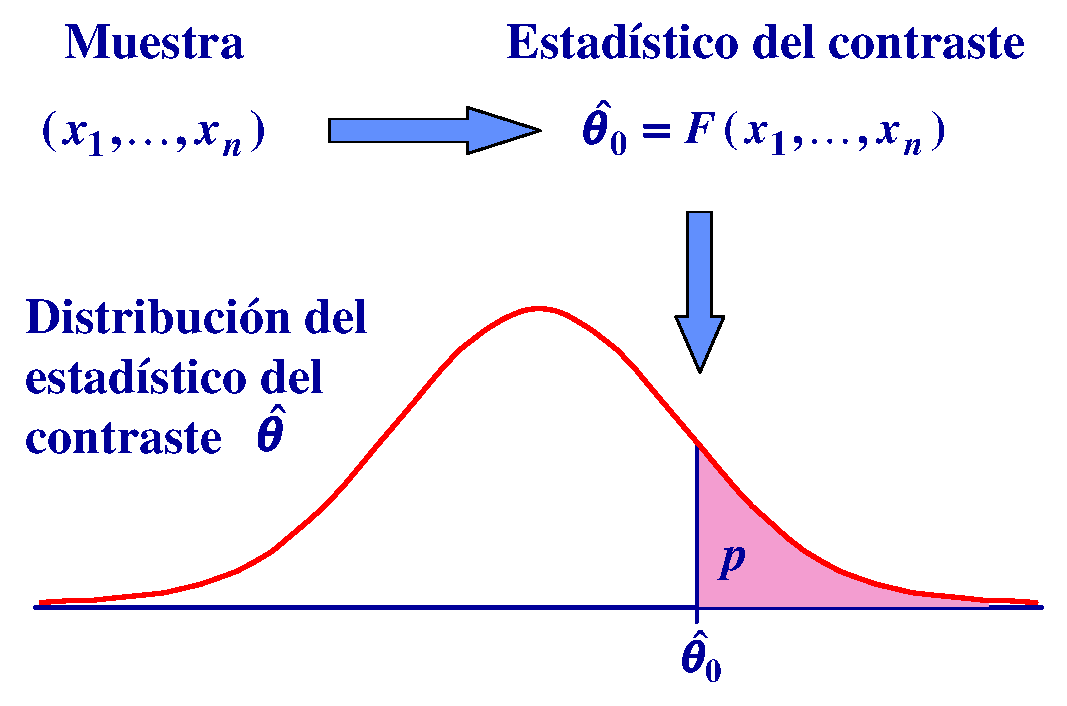
\includegraphics[scale=0.5]{contrastes/img/estadisticocontraste}
\caption{El $p$-valor de un contraste unilateral con cola a la derecha.}
\label{g:pvalor}
\end{center}
\end{figure}

Una vez calculado el $p$-valor, si hemos fijado el nivel de significación $\alpha$ y han quedado delimitadas las
regiones de aceptación y rechazo, el que la estimación caiga dentro de la región de rechazo es equivalente a que
$p<\alpha$, mientras que si cae dentro de la región de aceptación, entonces $p\geq \alpha$.
Esta forma de abordar los contrastes, nos da una visión más amplia, ya que nos da información de para qué niveles de
significación puede rechazarse la hipótesis nula, y para cuales no se puede.


\subsubsection{Contrastes y Estadísticos de Contraste}
Apoyándose en las distintas distribuciones en el muestreo comentadas en las prácticas sobre intervalos de confianza, a
continuación se presentan las fórmulas para los principales estadísticos de contraste.

\subsubsection{Contraste para la media de una población normal con varianza conocida}
\begin{itemize}
\item Hipótesis Nula: $H_0:\ \mu=\mu_0$
\item Estadístico del contraste:
\[
\dfrac{\overline{X}-\mu_0 }{\dfrac{\sigma }{\sqrt{n}}}
\]
que sigue una distribución normal tipificada, $N(0,1)$.
\end{itemize}
Este contraste también es válido para la media de una población no normal, siempre y cuando las muestras sean grandes
$(n\geq 30)$, con varianza conocida; y para la media de la diferencia de datos emparejados, siempre y cuando la variable
diferencia siga una distribución normal con varianza conocida, o una distribución cualquiera si la muestra es grande.

\subsubsection{Contraste para la media de una población normal con varianza desconocida}
\begin{itemize}
\item Hipótesis Nula: $H_0:\ \mu=\mu_0$
\item Estadístico del contraste:
\[
\dfrac{\overline{X}-\mu_0}{\dfrac{S_{n-1}}{\sqrt{n}}}
\]
que sigue una distribución $t$ de Student con $n-1$ grados de libertad, $T(n-1)$.
\end{itemize}
Este contraste también es válido para la media de una población no normal en muestras grandes $(n\geq 30)$, con varianza
desconocida; y para la media de la diferencia de datos emparejados, siempre y cuando la variable diferencia siga una
distribución normal con varianza desconocida, o una distribución cualquiera si la muestra es grande.

\subsubsection{Contraste para la proporción en muestras grandes y distribuciones simétricas (tanto $np$ como $n(1-p)$
deben ser mayores que 5)}
\begin{itemize}
\item Hipótesis Nula: $H_0:\ p=p_0$
\item Estadístico del contraste:
\[
\frac{{p - p_0 }}{{\sqrt {\frac{{p\left( {1 - p} \right)}}{n}} }}
\]
que sigue una distribución normal tipificada, $N(0,1)$.
\end{itemize}


\subsubsection{Contraste para la varianza de una población normal}
\begin{itemize}
\item Hipótesis Nula: $H_0:\ \sigma^2=\sigma_0^2$
\item Estadístico del contraste:
\[
\frac{{\left( {n - 1} \right)S_{n - 1} ^2 }}{{\sigma _0 ^2 }}
\]
que sigue una distribución Chi-cuadrado con $n-1$ grados de libertad.
\end{itemize}

\subsubsection{Contraste para la diferencia de medias de poblaciones normales con varianzas conocidas}
\begin{itemize}
\item Hipótesis Nula: $H_0:\ \mu_1=\mu_2$
\item Estadístico del contraste:
\[
\frac{{\overline X  - \overline Y }}{{\sqrt {\frac{{\sigma _1 ^2}}{{n_1 }} + \frac{{\sigma _2 ^2 }}{{n_2 }}} }}
\]
que sigue una distribución normal tipificada, $N(0,1)$.
\end{itemize}
Este contraste también es válido para la diferencia de medias de dos poblaciones no normales, siempre y cuando las
muestras sean grandes ($n_1\geq 30$ y $n_2\geq 30$), con varianzas conocidas.

\subsubsection{Contraste para la diferencia de medias de poblaciones normales con varianzas desconocidas}
\begin{itemize}
\item Hipótesis Nula: $H_0:\ \mu_1=\mu_2$
\item Estadístico del contraste:
\[
\frac{{\overline X  - \overline Y }}{{\sqrt {\frac{{S_{1,n_1-1} ^2}}{{n_1 }} + \frac{{S_{2,n_2-1} ^2 }}{{n_2 }}} }}
\]
que sigue una distribución t de Student con $\nu$ grados de libertad, donde $\nu$ es el número entero más próximo al
valor de la expresión:
\[
\dfrac{\left( \dfrac{s_{1,n_{1}-1}^{2}}{n_{1}}+\dfrac{s_{2,n_{2}-1}^{2}}{n_{2}}\right)
^{2}}{\dfrac{\left(\dfrac{s_{1,n_{1}-1}^{2}}{n_{1}}\right)^{2}}{n_{1}+1}+\dfrac{\left(
\dfrac{s_{2,n_{2}-1}^{2}}{n_{2}}\right) ^{2}}{n_{2}+1}}-2.
\]
\end{itemize}
Este contraste también es válido para la diferencia de medias de dos poblaciones no normales, siempre y cuando las
muestras sean grandes ($n_1\geq 30$ y $n_2\geq 30$), con varianzas desconocidas.

\subsubsection{Contraste para la diferencia de proporciones en muestras grandes y distribuciones simétricas ($n_1p_1$, $n_1(1-p_1)$, $n_2p_2$,
$n_2(1-p_2)$ deben ser mayores que 5)}
\begin{itemize}
\item Hipótesis Nula: $H_0:\ p_1=p_2$
\item Estadístico del contraste:
\[
\frac{{p_1  - p_2 }}{{\sqrt {\frac{{p_1 \left( {1 - p_1 }\right)}}{{n_1 }} + \frac{{p_2 \left( {1 - p_2 } \right)}}{{n_2}}} }}
\]
que sigue una distribución normal tipificada, $N(0,1)$.
\end{itemize}

\subsubsection{Contraste para la igualdad de varianzas de poblaciones normales}
\begin{itemize}
\item Hipótesis Nula: $H_0:\ \sigma_1^2=\sigma_2^2$
\item Estadístico del contraste:
\[
\frac{{S^2 _{1,n_1  - 1} }}{{S^2 _{2,n_2  - 1} }}
\]
que sigue una distribución F de Fisher con $n_1-1$ y $n_2-1$ grados de libertad.
\end{itemize}

\clearpage
\newpage

\section{Ejercicios resueltos}
\begin{enumerate}[leftmargin=*]
\item Para averiguar si en una determinada población existen menos hombres que mujeres se plantea un contraste de
hipótesis sobre la proporción de hombres que hay en la población: $H_0:\ p=0.5$ frente a $H_1:\ p<0.5$ y para ello se
toma una muestra aleatoria de 10 personas. 
Se pide:
\begin{enumerate}
\item Suponiendo cierta la hipótesis nula, ¿qué distribución sigue la variable que mide el número de hombres en la
muestra de tamaño 10?
\item Suponiendo cierta la hipótesis nula, ¿cuál es la probabilidad de que en la muestra se obtengan 0 hombres?
¿Se aceptaría la hipótesis nula en tal caso? 
Justificar la respuesta.
\begin{indicacion}
\begin{enumerate}
\item Seleccionar el menú \menu{Teaching > Distribuciones > Discretas > Binomial > Probabili\-dades acumuladas}.
\item En el cuadro de diálogo que aparece, introducir 0 en el campo \campo{Valor(es) de la variable}, 10 en el campo
\campo{Nº de repeticiones}, $0.5$ en el campo \campo{Probabilidad de éxito}, marcar la opción \opcion{Cola izquierda} y
hacer click en el botón \boton{Aceptar}.
\end{enumerate}
\end{indicacion}

\item Suponiendo cierta la hipótesis nula, si se decide rechazarla cuando en la muestra haya 2 o menos hombres, ¿cuál es
el riesgo de equivocarse?
\begin{indicacion}
\begin{enumerate}
\item Seleccionar el menú \menu{Teaching > Distribuciones > Discretas > Binomial > Probabili\-dades acumuladas}.
\item En el cuadro de diálogo que aparece, introducir 2 en el campo \campo{Valor(es) de la variable}, 10 en el campo
\campo{Nº de repeticiones}, $0.5$ en el campo \campo{Probabilidad de éxito}, marcar la opción \opcion{Cola izquierda} y
hacer click en el botón \boton{Aceptar}.
\end{enumerate}
\end{indicacion}

\item Si el máximo riesgo de error $\alpha$ que se tolera es $0.05$, ¿qué número de hombres en la muestra formarían la
región de rechazo de la hipótesis nula?
\begin{indicacion}
\begin{enumerate}
\item Seleccionar el menú \menu{Teaching > Distribuciones > Discretas > Binomial > Probabili\-dades acumuladas}.
\item En el cuadro de diálogo que aparece, introducir 1 en el campo \campo{Valor(es) de la variable}, 10 en el campo
\campo{Nº de repeticiones}, $0.5$ en el campo \campo{Probabilidad de éxito}, marcar la opción \opcion{Cola izquierda} y
hacer click en el botón \boton{Aceptar}.
\end{enumerate}
\end{indicacion}

\item Suponiendo que la proporción real de hombres en la población fuese de $0.4$, ¿cuál es la potencia del contraste
para la región de rechazo del apartado anterior?
\begin{indicacion}
\begin{enumerate}
\item Seleccionar el menú \menu{Teaching > Distribuciones > Discretas > Binomial > Probabili\-dades acumuladas}.
\item En el cuadro de diálogo que aparece, introducir 1 en el campo \campo{Valor(es) de la variable}, 10 en el campo
\campo{Nº de repeticiones}, $0.4$ en el campo \campo{Probabilidad de éxito}, marcar la opción \opcion{Cola izquierda} y
hacer click en el botón \boton{Aceptar}.
\end{enumerate}
\end{indicacion}

\item Si en lugar de una muestra de tamaño 10 se tomase una muestra de tamaño 100, y haciendo uso de la aproximación de
una distribución binomial mediante una normal, ¿qué número de hombres en la muestra formarían la región de rechazo para
un riesgo $\alpha=0.05$? 
¿Qué potencia tendría ahora el contraste si la proporción real de hombres fuese de $0.4$? 
¿Es mejor o peor contraste que el anterior? 
Justificar la respuesta.
\begin{indicacion}
Una distribución binomial $B(100,\, 0.5)$ puede aproximarse mediante una normal $N(50,5)$.
\begin{enumerate}
\item Seleccionar el menú \menu{Teaching > Distribuciones > Continuas > Normal > Cuantiles}.
\item En el cuadro de diálogo que aparece, introducir las probabilidad $0.05$ en el campo \campo{Probabilidades}, 50 en
el campo \campo{media}, 5 en el campo \campo{desviación típica}, marcar la opción \opcion{Cola izquierda} y hacer click
en el botón \boton{Aceptar}.
\end{enumerate}
El valor obtenido es la frontera entre la región de aceptación y la región de rechazo. 
Si en la muestra se obtienen menos hombres de dicho valor se rechazará la hipótesis nula, mientras que si se obtienen
más se aceptará. 
Para calcular la potencia de contraste:
\begin{enumerate}
\item Seleccionar el menú \menu{Teaching > Distribuciones > Continuas > Normal > Probabili\-dades acumuladas}.
\item En el cuadro de diálogo que aparece, introducir el valor de la frontera en el campo \campo{Valor(es) de la
variable}, 40 en el campo \campo{media}, $4.899$ en el campo \campo{desviación típica}, marcar la opción \opcion{Cola
izquierda} y hacer click en el botón \boton{Aceptar}.
\end{enumerate}
\end{indicacion}

\item Si se toma una muestra de tamaño 100 y se observan 41 hombres, ¿cuál es $p$-valor del contraste? 
¿Podría rechazarse la hipótesis nula pra un riesgo $\alpha=0.05$? 
¿y para un riesgo $\alpha=0.01$?
\begin{indicacion}
\begin{enumerate}
\item Seleccionar el menú \menu{Teaching > Test paramétricos > Proporciones > Test para una proporción}.
\item En el cuadro de diálogo que aparece marcar la casilla de \opcion{Introducción manual de frecuencias}, introducir
41 en el campo \campo{Frecuencia muestral} e introducir 100 en el campo \campo{Tamaño muestral}.
\item En la solapa \menu{Opciones de contraste}, introducir $0.5$ en el campo \campo{Hipótesis nula}, seleccionar
como hipótesis alternativa \opcion{Unilateral menor} y hacer click en el botón \boton{Aceptar}.
\end{enumerate}
\end{indicacion}
\end{enumerate}


\item  Se analiza la concentración de principio activo en una muestra de 10 envases tomados de un lote de un fármaco, obteniendo los
siguientes resultados en mg/mm$^{3}$: 
\[ 
17.6-19.2-21.3-15.1-17.6-18.9-16.2-18.3-19.0-16.4 
\]
Se pide:
\begin{enumerate}
\item Crear un conjunto de datos con la variable \variable{concentracion}.

\item Realizar el contraste de hipótesis bilateral: $H_0$: $\mu=18$ y $H_1$: $\mu\neq18$ con un nivel de significación
$0.05$.
\begin{indicacion}
\begin{enumerate}
\item Seleccionar el menú \menu{Teaching > Test paramétricos > Medias > Test t para una muestra}.
\item En el cuadro de diálogo que aparece seleccionar la variable \variable{concentracion}.
\item En la solapa \menu{Opciones de contraste}, introducir 18 en el campo \campo{Hipótesis nula}, seleccionar como
hipótesis alternativa la opción \opcion{Bilateral} y hacer click sobre el botón \boton{Aceptar}.
\end{enumerate}
\end{indicacion}

\item De igual manera realizar los contrastes bilaterales: $H_0$: $\mu=19.5$ y $H_1$: $\mu\neq19.5$ con un niveles de
significación $0.05$ y $0.01$.
¿Cómo afecta la disminución en el nivel de significación en la facilidad para rechazar $H_0$?

\begin{indicacion}Seguir los mismos pasos del apartado anterior introduciendo $19.5$ en el campo \campo{Hipótesis nula}.
\end{indicacion}

\item Realizar los contrastes bilaterales y unilaterales para la hipótesis nula $H_0$: $\mu=17$ con un nivel de significación de $0.05$.
¿Qué relación hay entre el $p$-valor de los contrastes bilateral y unilaterales?
\begin{indicacion}
\begin{enumerate}
\item Seleccionar el menú \menu{Teaching > Test paramétricos > Medias > Test t para una muestra}.
\item En el cuadro de diálogo que aparece seleccionar la variable \variable{concentracion}.
\item En la solapa \menu{Opciones de contraste}, introducir 17 en el campo \campo{Hipótesis nula}, seleccionar como
hipótesis alternativa \opcion{Bilateral} y hacer click sobre el botón \boton{Aceptar}.
\item Para el contraste de menor repetir lo mismo seleccionando como hipótesis alternativa \opcion{Unilateral menor}.
\item Para el contraste de mayor repetir lo mismo seleccionando como hipótesis alternativa \opcion{Unilateral mayor}.
\end{enumerate}
\end{indicacion}

\item Si el fabricante del lote asegura haber aumentado la concentración de principio activo con respecto a anteriores
lotes, en los que la media era de 17 mg/mm$^3$, ¿se acepta o se rechaza la afirmación del fabricante?

\item ¿Cuál sería el tamaño muestral requerido para poder detectar una diferencia de $0.5$ mg/mm$^{3}$ más con un nivel de
significación $\alpha=0.05$ y una potencia $1-\beta=0.8$?
\begin{indicacion}
Para calcular el tamaño muestral se necesita saber la desviación típica de la población o una estimación suya. 
Para ello se calcula previamente la cuasivarianza muestral
\begin{enumerate}
\item Seleccionar el menú \menu{Teaching > Estadística descriptiva > Estadísticos}.
\item En el cuadro de diálogo que aparece seleccionar la variable \variable{concentracion}.
\item En la solapa \menu{Estadísticos básicos} marcar la opción \opcion{Cuasidesviación típica} y hacer click en el
botón \boton{Aceptar}.
\end{enumerate}
Para calcular el tamaño muestral:
\begin{enumerate}
\item Seleccionar el menú \menu{Teaching > Test paramétricos > Medias > Cálculo del tamaño muestral para el test T}.
\item En el cuadro de diálogo que aparece introducir en el campo \campo{Diferencia en las medias} el valor 0.5,
introducir en el campo \campo{Desviación típica} el valor de la cuasivesviación típica obtenido, introducir el valor
$0.05$ en el campo \campo{Nivel de significación}, introducir el valor $0.8$ en el campo \campo{Potencia}, marcar la
opción \opcion{Una muestra} en el campo \campo{Tipo de test}, seleccionar como hipótesis alternativa \opcion{Unilateral}
y hacer click sobre el botón \boton{Aceptar}.
\end{enumerate}
\end{indicacion}
\end{enumerate}


\item En una encuesta realizada en una facultad, sobre si el alumnado utiliza habitualmente (al menos una vez a la
semana) la biblioteca de la misma, se han obtenido los siguientes resultados:
\begin{flushleft}
\begin{tabular}{|l|l|l|l|l|l|l|l|l|l|l|l|l|l|l|l|l|l|}
\hline
Alumno & 1 & 2 & 3 & 4 & 5 & 6 & 7 & 8 & 9 & 10 & 11 & 12 & 13 & 14 & 15 & 16 & 17 \\
\hline
Respuesta & no & si & no & no & no & si & no & si & si & si & si & no & si & no & si & no & no \\
\hline
\end{tabular}
\newline

\begin{tabular}{|l|l|l|l|l|l|l|l|l|l|l|l|l|l|l|l|l|l|}
\hline
Alumno & 18 & 19 & 20 & 21 & 22 & 23 & 24 & 25 & 26 & 27 & 28 & 29 & 30 & 31 & 32 & 33 & 34 \\
\hline
Respuesta & no & si & si & si & no & no & si & no & no & si & si & no & no & si & no & si & no \\
\hline
\end{tabular}
\end{flushleft}

\begin{enumerate}
\item Crear un conjunto de datos con la variable \variable{respuesta} como factor.

\item Contrastar si el porcentaje de alumnos que utiliza regularmente la biblioteca es superior al 40\%. 
\begin{indicacion}
\begin{enumerate}
\item Seleccionar el menú \menu{Teaching > Test paramétricos > Proporciones > Test para una proporción}.
\item En el cuadro de diálogo que aparece seleccionar la variable \variable{respuesta} e introducir \texttt{Si} en el campo \campo{Categoría}.
\item En la solapa \menu{Opciones de contraste}, introducir $0.4$ en el campo \campo{Hipótesis nula}, seleccionar como
hipótesis alternativa \opcion{Unilateral mayor} y hacer click en el botón \boton{Aceptar}.
\end{enumerate}
\end{indicacion}
\end{enumerate}

\item Varios investigadores desean saber si es posible concluir que dos poblaciones de niños difieren respecto a la edad
promedio en la cual pueden caminar por sí solos.
Los investigadores obtuvieron los siguientes datos para la edad al comenzar a andar (expresada en meses):
\begin{center}
\begin{tabular}{ll}
Muestra en la población $A$: & $9.5-10.5-9.0-9.8-10.0-13.0-10.0-13.5-10.0-9.8$\\
Muestra en la población $B$: & $12.5-9.5-13.5-13.8-12.0-13.8-12.5-9.5-12.0-13.5-12.0-12.0$
\end{tabular}
\end{center}

\begin{enumerate}
\item Crear un conjunto de datos con las variables \variable{población} y \variable{edad}.

\item Realizar un contraste de hipótesis con un nivel de significación de $0.05$ para dar respuesta a la conclusión que
buscan los investigadores.
\begin{indicacion}
Primero hay que realizar un constraste de comparación de varianzas.
\begin{enumerate}
\item Seleccionar el menú \menu{Teaching > Test paramétricos > Varianzas > Test F para dos varianzas}.
\item En el cuadro de dialogo que aparece seleccionar la variable \variable{edad} en el campo \campo{Comparar} y la
variable \variable{población} en el campo \campo{Según}.
\item En la solapa \menu{Opciones de contraste} seleccionar como hipótesis alternativa \opcion{Bilateral} y hacer click
sobre el botón \boton{Aceptar}.
\end{enumerate}
Se mantiene la hipótesis de igualdad de varianzas con la confianza fijada si el el $p$-valor es mayor que $0.5$. 
Después se realiza el contraste de comparación de medias.
\begin{enumerate}
\item Seleccionar el menú \menu{Teaching > Test paramétricos > Medias > Test t para dos muestras independientes}.
\item En el cuadro de dialogo que aparece seleccionar la variable \variable{edad} en el campo \campo{Comparar} y la
variable \variable{población} en el campo \campo{Según}.
\item En la solapa \menu{Opciones de contraste} seleccionar como hipótesis alternativa \opcion{Bilateral},
marcar la casilla \opcion{Suponer varianzas iguales} y hacer click sobre el botón \boton{Aceptar}.
\end{enumerate}
Hay diferencias entre las poblaciones si el $p$-valor es menor que $0.05$.
\end{indicacion}
\end{enumerate}


\item Algunos investigadores han observado una mayor resistencia de las vías respiratorias en fumadores que en no
fumadores.
Para confirmar dicha hipótesis, se realizó un estudio para comparar el porcentaje de retención traqueobronquial en las
mismas personas cuando aún eran fumadoras y transcurrido un año después de dejarlo.
Los resultados se indican en la tabla siguiente:
\[
\begin{array}{cc}
\hline
\multicolumn{2}{c}{\text{Porcentaje de retención}} \\
\hline
\text{Cuando fumaba} & \text{Transcurrido un año sin fumar} \\
\hline
60.6 & 47.5 \\
12.0 & 13.3 \\
56.0 & 33.0 \\
75.2 & 55.2 \\
12.5 & 21.9 \\
29.7 & 27.9 \\
57.2 & 54.3 \\
62.7 & 13.9 \\
28.7 & 8.90 \\
66.0 & 46.1 \\
25.2 & 29.8 \\
40.1 & 36.2 \\
\hline
\end{array}
\]

\begin{enumerate}
\item Crear un conjunto de datos con las variables \variable{antes} y \variable{después} e introducir los datos.

\item Plantear el contraste de hipótesis adecuado para confirmar o denegar la hipótesis de los investigadores. 
\begin{indicacion}
\begin{enumerate}
\item Seleccionar el menú \menu{Teaching > Test paramétricos > Medias > Test t para dos muestras pareadas}.
\item En el cuadro de diálogo que aparece seleccionar la variable \variable{antes} en el campo \campo{Comparar} y la variable
\variable{después} en el campo \campo{Con}.
\item En la solapa \menu{Opciones de contraste} seleccionar como hipótesis alternativa \opcion{Unilateral mayor} y hacer
click en el botón \boton{Aceptar}.
\end{enumerate}
\end{indicacion}
\end{enumerate}


\item Un profesor universitario ha tenido dos grupos de clase a lo largo del año: uno con horario de mañana y otro de
tarde. En el de mañana, sobre un total de 80 alumnos, han aprobado 55; y en el de tarde, sobre un total de 90 alumnos,
han aprobado 32. 
¿Se puede afirmar que hay diferencias significativas entre los porcentajes de aprobados en ambos grupos? 
Justificar la respuesta.
\begin{indicacion}
\begin{enumerate}
\item Seleccionar el menú \menu{Teaching > Test paramétricos > Proporciones > Test para dos proporciones}, marcar la casilla \opcion{Introducción manual de frecuencias}, introducir 55 en el campo \campo{Frecuencia muestral 1}, introducir 80 en el campo
\campo{Tamaño muestral 1}, introducir 32 en el campo \campo{Frecuencia muestral 2} e introducir 90 en el campo
\campo{Tamaño muestral 2}.
\item En la solapa \menu{Opciones de contraste}, seleccionar como hipótesis alternativa \opcion{Bilateral} y hacer click
en el botón \boton{Aceptar}.
\end{enumerate}
\end{indicacion}

\end{enumerate}


\section{Ejercicios propuestos}
\begin{enumerate}[leftmargin=*] 
\item El fichero \texttt{pulso.txt} contiene información sobre el pulso de un grupo de pacientes que han realizado
distintos ejercicios:
pulso en reposo (pulse1), pulso después de hacer ejercicio (pulse2), tipo de ejercicio (ran, 1=correr, 2=andar), sexo
(sex, 1=hombre, 2=mujer) y peso (weight).
Se pide:
\begin{enumerate}
\item Contrastar si el pulso en reposo está por debajo de 75 pulsaciones.
\item ¿Qué tamaño muestral sería necesario para detectar una diferencia de 2 pulsaciones más en la media de las
pulsaciones en reposo, con un nivel de significación $0.05$ y una potencia de $0.9$?
\item Contrastar si el pulso después de correr está por encima de 85 pulsaciones.
\item Contrastar si el porcentaje de personas con taquicardia leve (número de pulsaciones en reposo por encima de 90)
supera el 5\%.
\item ¿Se puede afirmar que el ejercicio aumenta las pulsaciones con una significación de $0.05$? 
¿y con una significación $0.01$?
Justificar la respuesta.
\item ¿Existen diferencias entre las pulsaciones después de andar y después de correr? Justificar la respuesta.
\item ¿Existen diferencias entre las pulsaciones en reposo entre hombres y mujeres? 
¿Y entre las pulsaciones después de correr? Justificar la respuesta.
\end{enumerate}

\end {enumerate}
